\documentclass[12pt]{article}
\usepackage[utf8]{inputenc}
\usepackage{pgf,tikz,pgfplots}
\pgfplotsset{compat=1.15}
\usepackage{mathrsfs}
\usetikzlibrary{arrows}
\usepackage{fontspec}
\setmainfont[Renderer=ICU,Mapping=tex-text]{Cousine}
\usepackage{amssymb}
\usepackage[paperwidth=13.2cm,paperheight=22.7cm,left=0.1cm,right=0.1cm,top=0.1cm,bottom=0.1cm]{geometry}
\begin{document}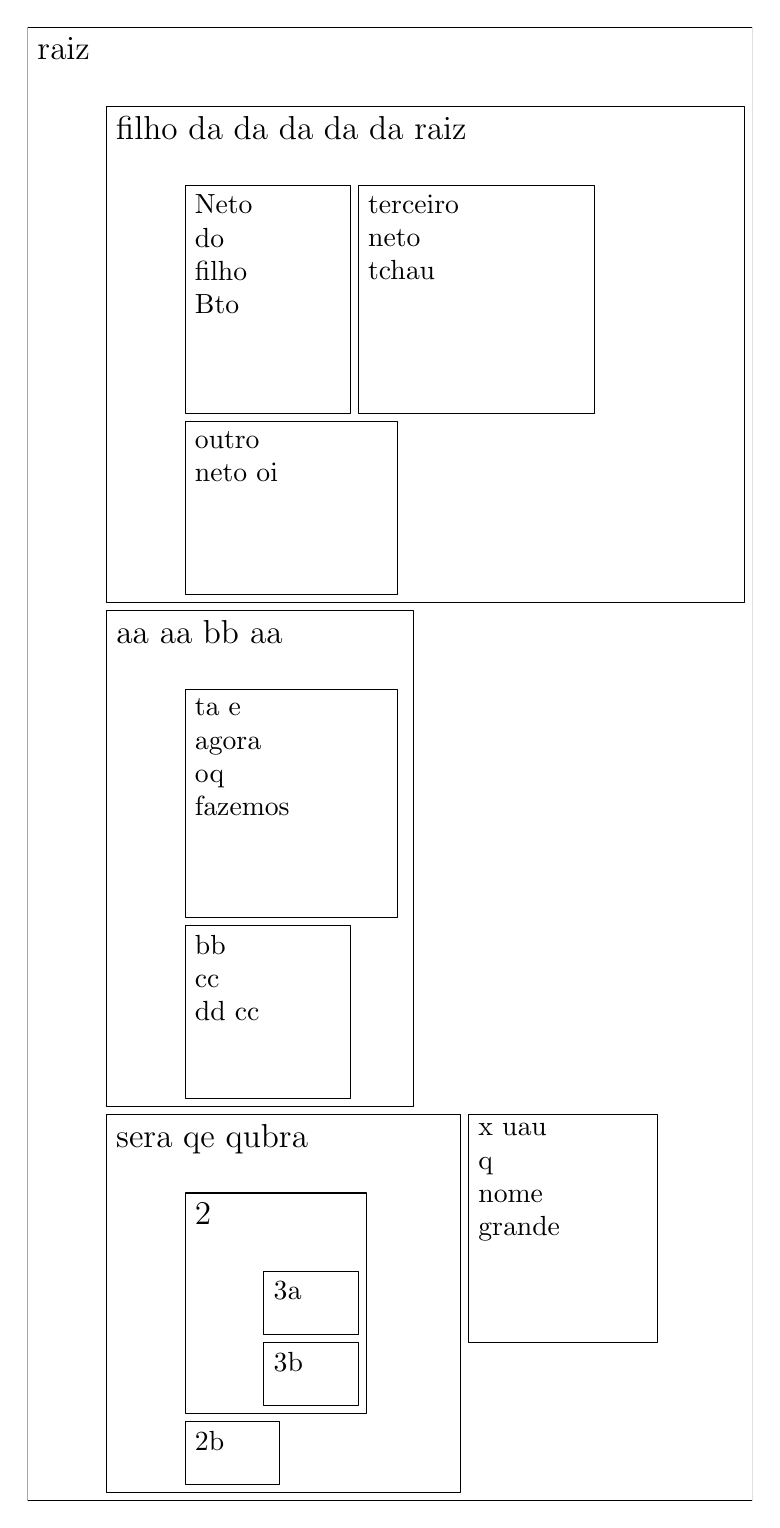
\begin{tikzpicture}[line cap=round,line join=round,>=triangle 45,x=1cm,y=1cm]
\clip(0, 0)rectangle(9.2, -18.7);

\draw(0, 0) node[anchor=north west] { \large raiz};
\draw (0, 0) rectangle (9.2,-18.7);
\draw(1, -1) node[anchor=north west] { \large filho da da da da da raiz};
\draw (1, -1) rectangle (9.1,-7.299999999999999);
\draw(2, -2) node[anchor=north west,align=left] {Neto\\ do\\ filho\\ Bto};
\draw (2, -2) rectangle (4.1,-4.9);
\draw(4.2, -2) node[anchor=north west,align=left] {terceiro\\ neto\\ tchau};
\draw (4.2, -2) rectangle (7.2,-4.9);
\draw(2, -5.0) node[anchor=north west,align=left] {outro\\ neto oi};
\draw (2, -5.0) rectangle (4.7,-7.199999999999999);
\draw(1, -7.399999999999999) node[anchor=north west] { \large aa aa bb aa};
\draw (1, -7.399999999999999) rectangle (4.9,-13.699999999999998);
\draw(2, -8.399999999999999) node[anchor=north west,align=left] {ta e\\ agora\\ oq \\ fazemos};
\draw (2, -8.399999999999999) rectangle (4.7,-11.299999999999999);
\draw(2, -11.399999999999999) node[anchor=north west,align=left] {bb\\ cc\\ dd cc};
\draw (2, -11.399999999999999) rectangle (4.1,-13.599999999999998);
\draw(1, -13.799999999999997) node[anchor=north west] { \large sera qe qubra};
\draw (1, -13.799999999999997) rectangle (5.5,-18.599999999999998);
\draw(2, -14.799999999999997) node[anchor=north west] { \large 2};
\draw (2, -14.799999999999997) rectangle (4.300000000000001,-17.599999999999998);
\draw(3, -15.799999999999997) node[anchor=north west,align=left] {3a};
\draw (3, -15.799999999999997) rectangle (4.2,-16.599999999999998);
\draw(3, -16.699999999999996) node[anchor=north west,align=left] {3b};
\draw (3, -16.699999999999996) rectangle (4.2,-17.499999999999996);
\draw(2, -17.699999999999996) node[anchor=north west,align=left] {2b};
\draw (2, -17.699999999999996) rectangle (3.2,-18.499999999999996);
\draw(5.6, -13.799999999999997) node[anchor=north west,align=left] {x uau\\ q\\ nome\\ grande};
\draw (5.6, -13.799999999999997) rectangle (8.0,-16.699999999999996);
\end{tikzpicture}

\end{document}